\section{Steering Model of the Vehicle}\label{sec:SteeringModel}
The following section will describe and model the steering of the vehicle. The relation between the PWM sent to the servo and the actual steering of the vehicle will be found. A overview of the braking system can be seen in \figref{steeringMechanical}.

 \begin{figure}[H]
 	\centering
 	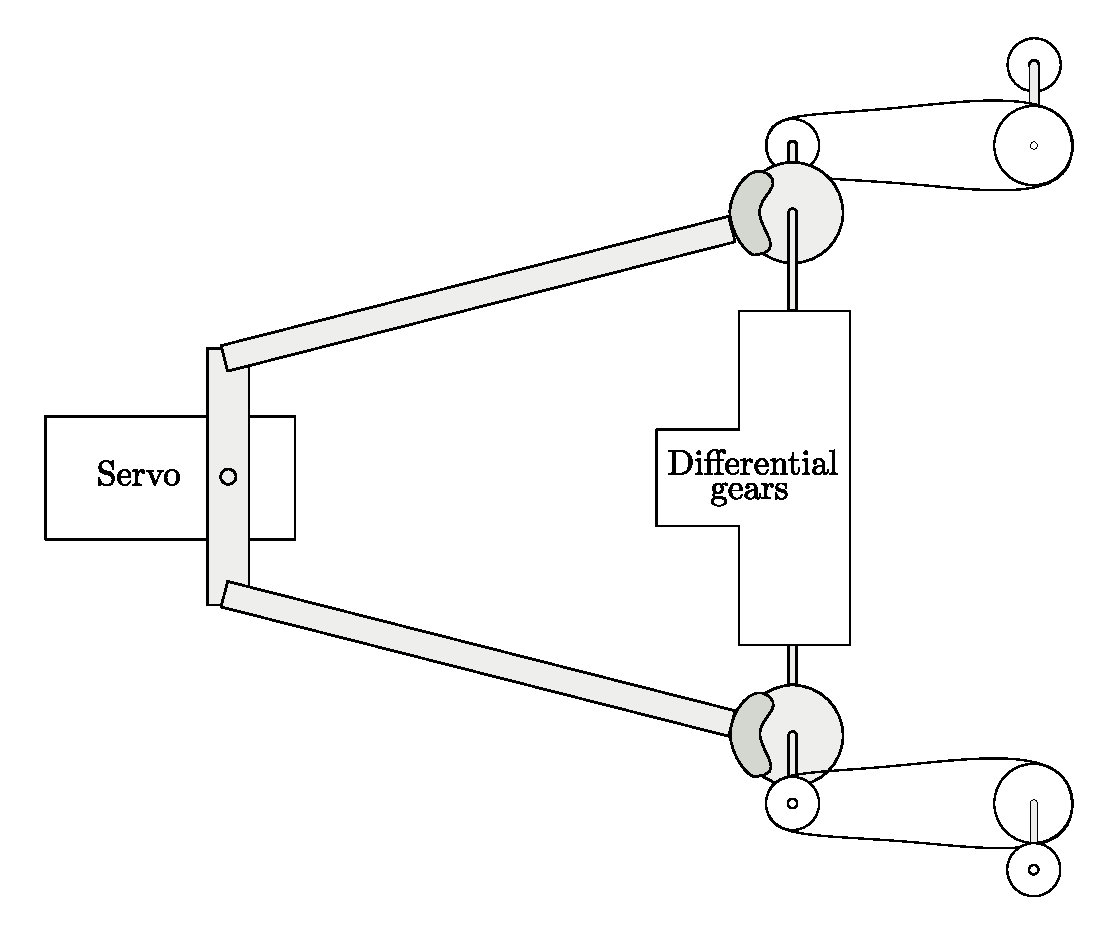
\includegraphics[scale=0.6]{figures/steeringMechanical.pdf}
 	\caption{Mechanical drawing of the steering}
 	\label{steeringMechanical}
 \end{figure}

When the servo turns one way, it push the brake pads on the brake disc, to add a friction. The differential gears will transfer the power from one belt to the other if one brake is triggered.

\subsection{Steering Parameters}
 To obtain a steering model everything in the system between the input and the output is black boxed. Second or first order, if it is second the black box should be expanded, if it is first there is no need because then we have all the parameters from the test.
 
 figure of the black box
 \begin{figure}[H]
 	\centering
 	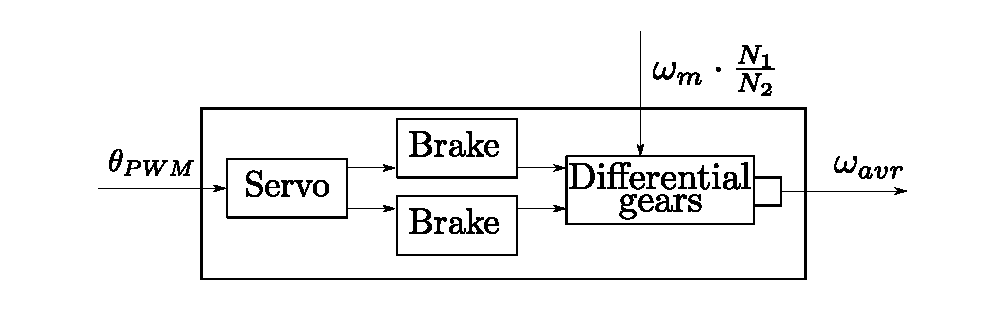
\includegraphics[scale=1]{figures/steeringDiagramBlackBox.pdf}
 	\caption{A diagram showing the black box}
 	\label{steeringDiagramBlackBox}
 \end{figure}
 
 appendix
 
show that it's a first order system\\
then integrator\\
then is linear(multiples values) the speed of turning at different PWM angle of the servo?
